\chapter{Interacciones y movimiento}

 
\section{Diagramas mostrando cambios de velocidad}

Está parte de la notas está basada en el libro Matter \& Interactions \cite{MI}

En diagramas físicos la velocidad de un objeto es representada por un
vector: una línea con una flecha. La cola de la flecha se coloca donde
el objeto está localizado, y la punta de la flecha en la dirección del
movimiento del objeto. La longitud de la flecha es proporcional a la
rapidez del objeto. De este modo la velocidad se describe como un
vector. A la magnitud de la velocidad se le llama rapidez.

\subsection{Movimiento uniforme}
Suponga que observa una roca moviéndose en el espacio exterior
bastante alejada de cualquier objeto. No sabemos que la hizo mover la
primera vez; presumiblemente hace mucho tiempo una interacción le dio
alguna velocidad y esta ha estado moviéndose desde entonces en el
espacio vacío.

Es un hecho observacional que tal objeto aislado se mueve con una
rapidez constante (que no cambia), en una línea recta. Su velocidad no
cambia (ni su dirección ni su rapidez
\begin{figure}
  \centering
  \includegraphics[scale=0.2]{uniform}
  \caption{Movimiento uniforme: sin cambio en la rapidez o la dirección.}
  \label{fig:uniform}
\end{figure}
cambia). A tal movimiento con
velocidad constante le llamaremos movimiento uniforme y es ilustrado
en la figura~\ref{fig:uniform}

Si observamos un electrón cambiando la dirección de su velocidad,
podemos atribuirlo al efecto de repulsión de un electrón cercano como
se muestra en la figura~\ref{fig:repulsion2} (a). Mientras que si el
electrón se está acelerando en línea recta, cambiando la magnitud de
su velocidad pero manteniendo la dirección, lo podemos atribuir a otro
electrón a lo largo de su línea de movimiento como se muestra en la
figura~\ref{fig:repulsion2} (b)
\begin{figure}
  \centering
  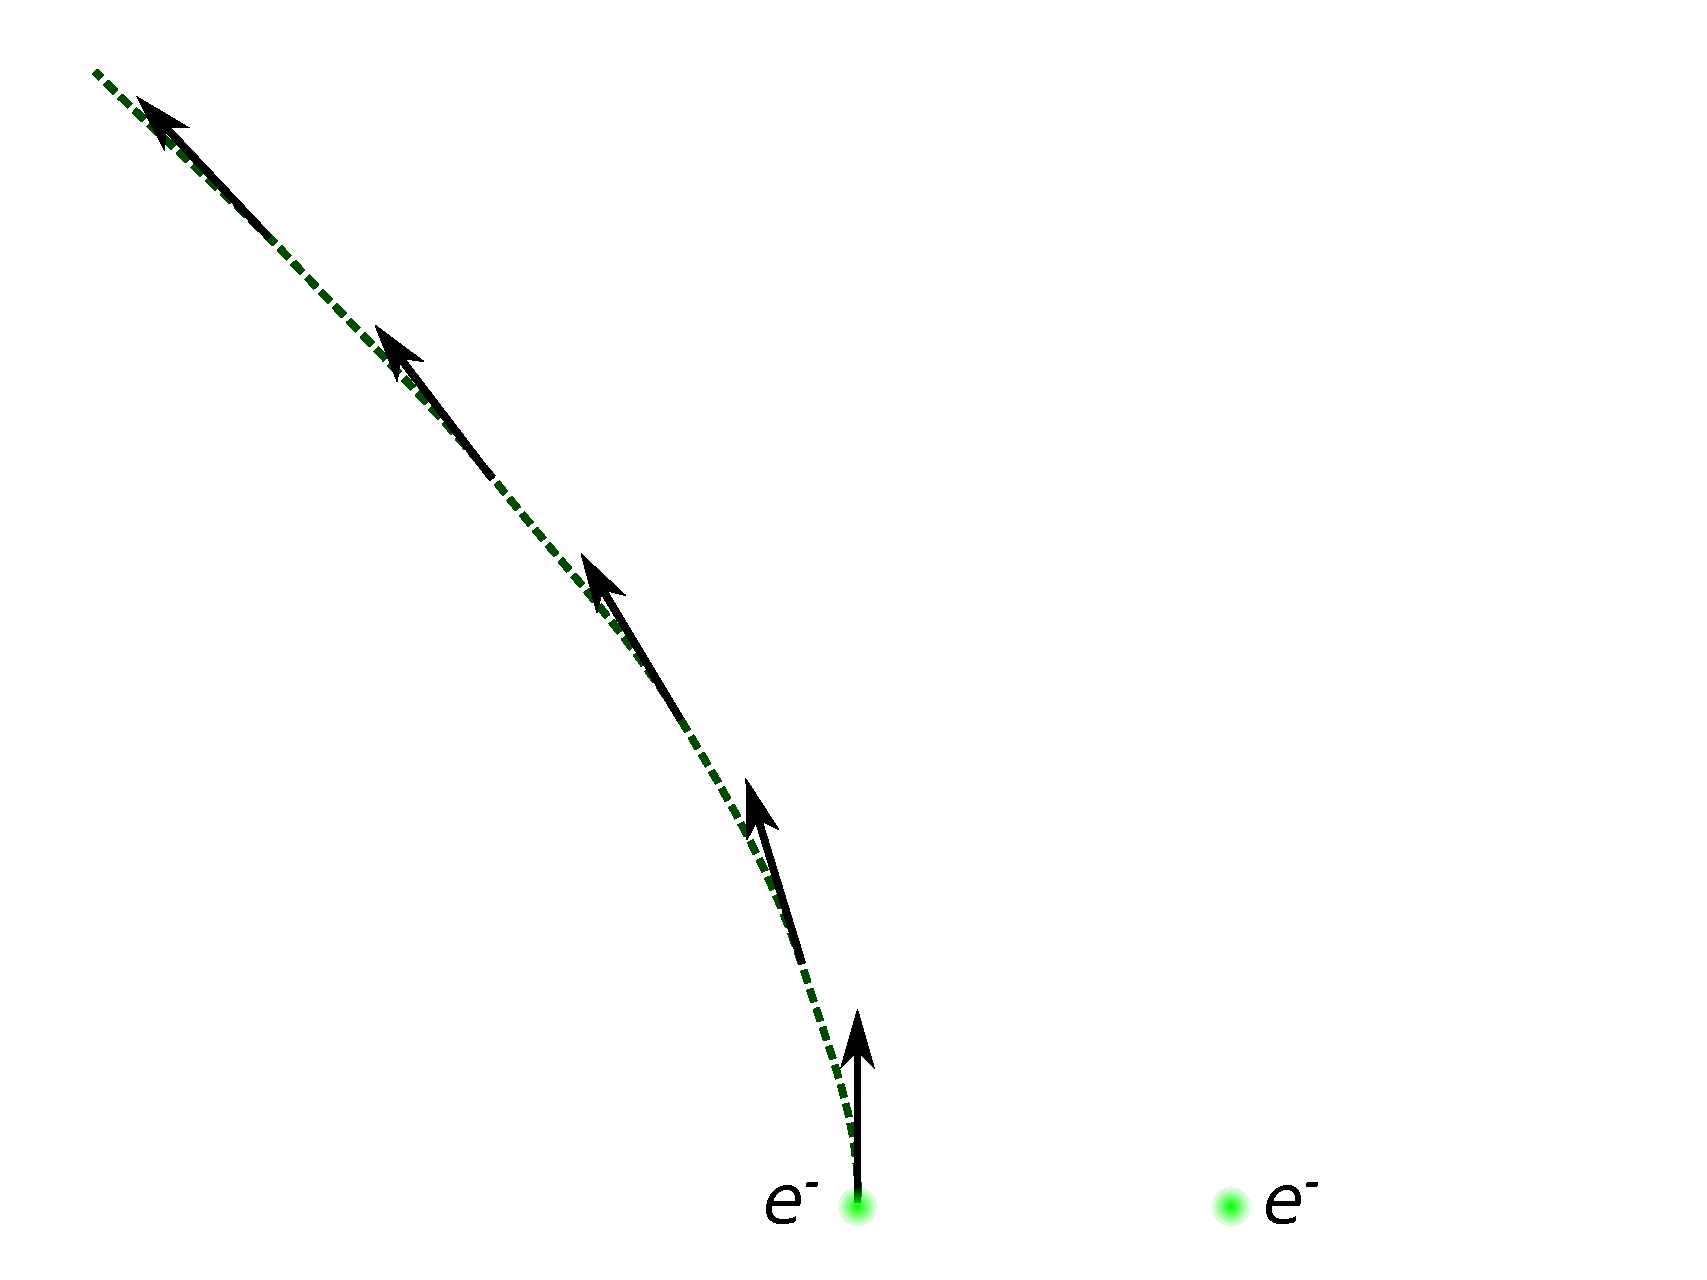
\includegraphics[scale=0.3]{repulsion2} 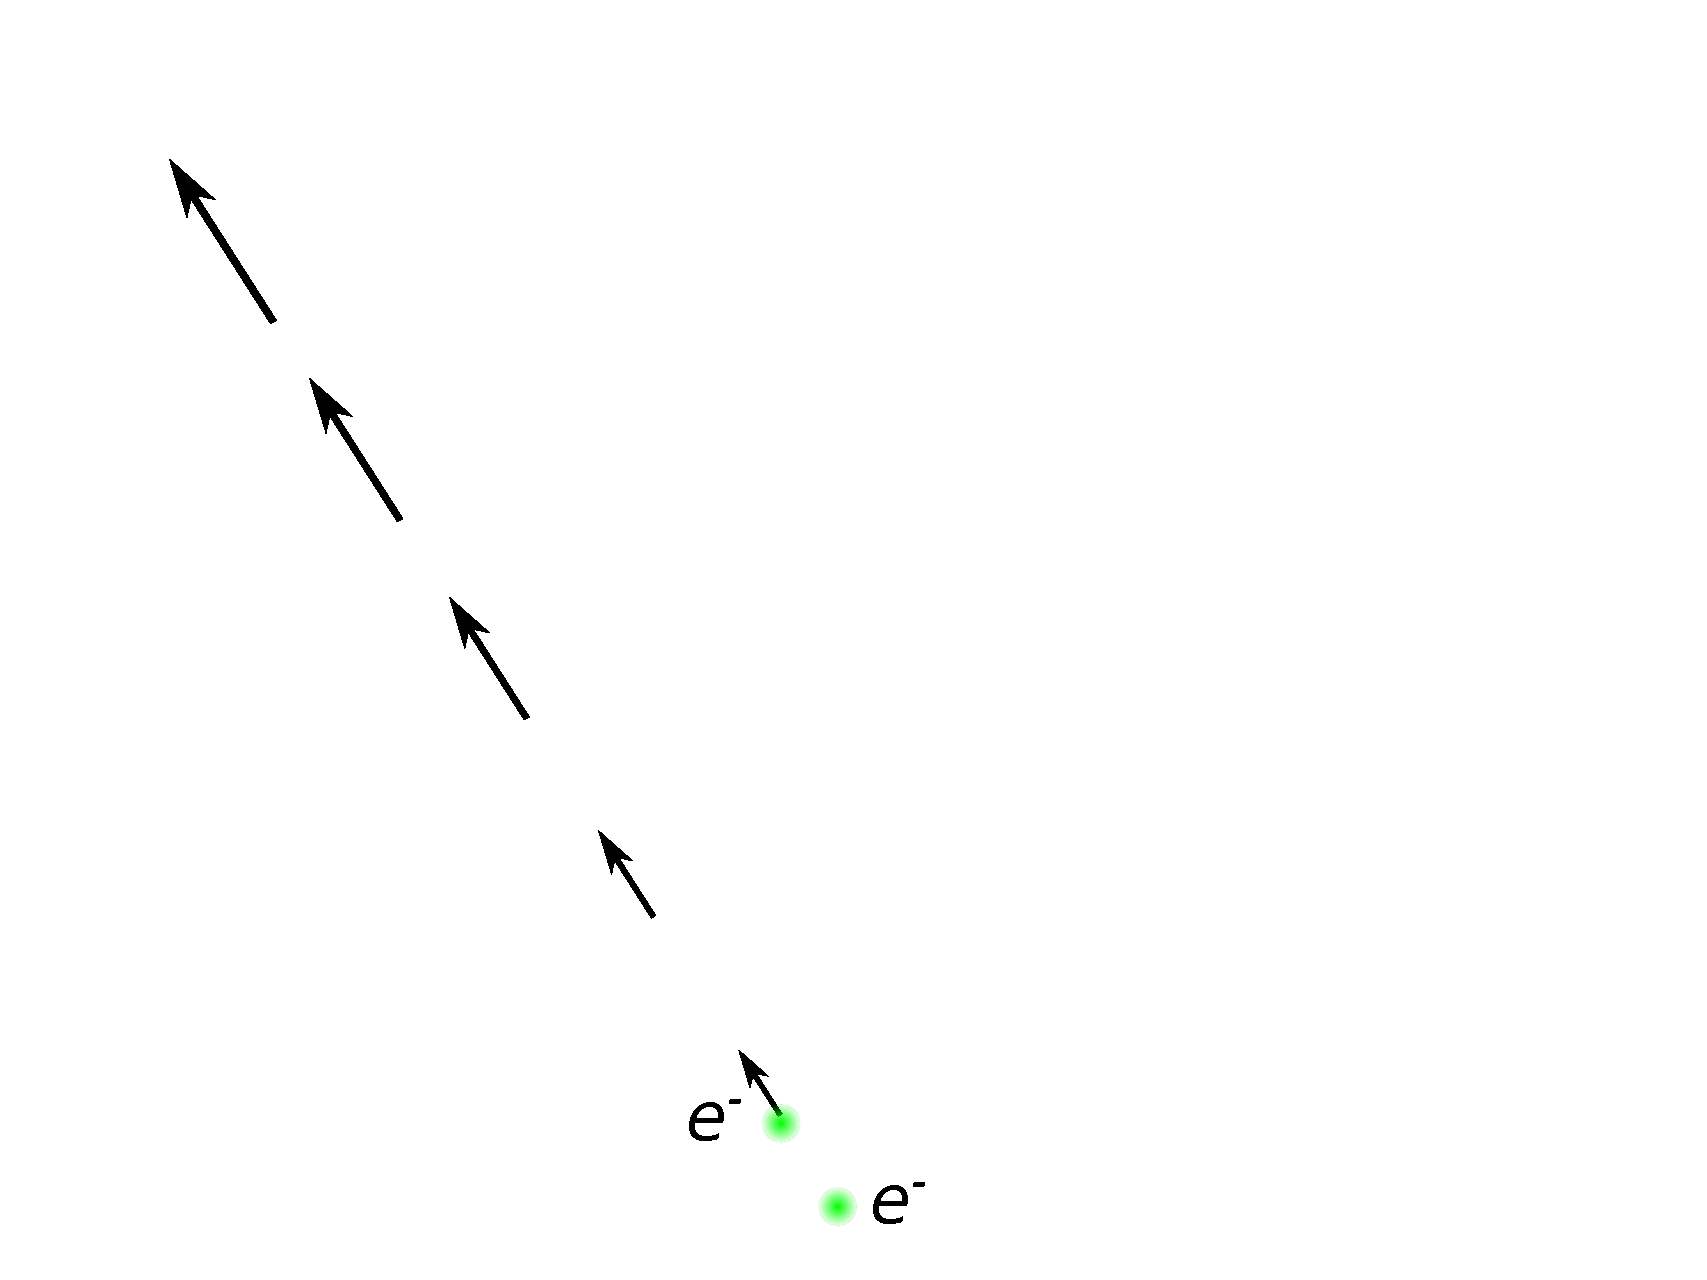
\includegraphics[scale=0.3]{repulsion4}\\
    (a) \hspace{5cm} (b)
  \caption{Cambio en dirección}
  \label{fig:repulsion2}
\end{figure}

Podemos establecer entonces,

\begin{frame}
  \begin{block}{Primera Ley de Newton:}
    Un objeto se mueve en línea recta y a una rapidez constante
    excepto en la medida que interaccione con otros objetos
  \end{block}
\end{frame}

Antes de la Primera Ley de Newton,  se pensaba que se requería un empuje constante para mantener algo en movimiento. Con La Primera Ley de Newton, o Ley de Inercia, ¡No se necesitan interacciones para que algo se mueva! (o, como veremos luego, rote)


Para mantener una silla moviéndose a velocidad constante hay que estar empujándola todo el tiempo. La primera Ley de Newton ¿implicaría que la silla se debe mover a velocidad constante sin que nadie la esté empujando? ¿El empuje constante debería cambiar la dirección o la rapidez del movimiento? ¿está situación de la vida diaria viola la primera ley de Newton?

El factor que complica la situación es que sus manos no son lo único
que interacciona con la silla. El piso también interacciona con la
silla en una forma que llamamos fricción. Si se empuja la silla lo
suficiente como para compensar \emph{exactamente} la fricción, la suma
total de las interacciones es \emph{cero}, y la silla se mueve a
velocidad constante como lo predice la primera ley de Newton. Si el
empuje es más fuerte que la fuerza que hace el piso, entonces la
rapidez de la silla se debe incrementar.


Es muy difícil observar movimiento sin fricción en la vida diaria, debido a que los objetos interaccionan con otros objetos incluyendo el aire, superficies, etc. Esto explica porque le tomo a la gente tanto tiempo entender claramente la relación entre interacción y cambio (Newton nación en 1542).

\begin{frame}
Ejemplos de baja fricción
\begin{itemize}
\item Un disco de hockey deslizándose sobre el hielo.
\item Un tren sobre los rieles de acero.
\item Un tren de levitación magnética a bajas velocidades.
\item Un tren de levitación magnética moviéndose a lo largo de un tubo de vacío.
\item Un objeto en el espacio exterior lejos de cualquier otro objeto.
\end{itemize}
\end{frame}

\ejemplo{}
\begin{frame}
  De acuerdo a la primer ley de Newton, ¿cuales de las siguientes frases sobre el movimiento de una nave después de apagada son correctas?
  \begin{enumerate}
  \item La nave se moverá en línea recta
    \label{item:n1}
  \item La nave viajará en una trayectoria curva
  \item La nave entrará en una orbita circular
  \item La velocidad de la nave no cambiará
    \label{item:n2}
  \item La nave se detendrá gradualmente
  \item La nave parará de inmediato
  \end{enumerate}
\end{frame}

Las frases correctas son  \ref{item:n1}. y \ref{item:n2}.\finejemplo

Incluso en presencias de fricción el reposo es algo relativo al observador. Un borrador en reposo sobre una mesa está en reposo relativo para los observadores en el salón, pero no para un observador en la luna, el sol, el centro de la galaxia, etc.


La humanidad tardó aún mucho más tiempo en determinar cuales de las fuerzas en la naturaleza eran fundamentales y cuales eran resultaban por el efecto combinando de interacciones fundamentales.

Hoy sabemos que en la naturaleza existen cuatro interacciones fundamentales
\begin{itemize}
\item Interacción gravitacional.
\item Interacción electromagnética.
\item Interacción débil.
\item Interacción fuerte.
\end{itemize}

Las demás fuerzas como la fuerza nuclear, la fuerzas de Van der Waals, la fricción, la viscosidad, etc., son remanentes de la interacciones fundamentales. 

%Ver presentación sobre Interacciones y movimiento donde se establece la Primera Ley de Newton en la página del curso.

\section{Velocidad}

\subsection{Rapidez promedio}
La rapidez es la magnitud del vector velocidad, $\mathbf{v}$,  y por consiguiente es una cantidad escalar:

\begin{align}
  \label{eq:27}
\bar{v}=|\mathbf{v}|=\frac{d}{t}\,,
\end{align}
donde $\bar{v}$ es la \emph{rapidez promedio}, $d$ es la distancia
recorrida durante un tiempo $t$. En SI (Système Internationale) de
unidades, la rapidez promedio se mide en metros por segundo, y se
abrevia con $\si{\meter\per\second}$.

De \eqref{eq:27}
\begin{align}
  \label{eq:26}
  d=&\bar{v} t\nonumber\\
  t=&\frac{d}{\bar{v}}\,.
\end{align}

Es importante notar que las ecuaciones \eqref{eq:26} son dimensionalmente correctas, por ejemplo
\begin{align}
  [d]=&  \left[\bar{v}   \right] [t]\nonumber\\
  L=&\frac{L}{T}\times T\nonumber\\
  L=&L\,.
\end{align}

\subsection{Rapidez instantánea comparada a rapidez promedio}

Si un carro se mueve a $70\ \text{Km/h}$ (kilometros por hora) durante la primera hora y a $\SI{30}{\kilo\meter\per\hour}$
durante la segunda hora, este recorre en total $\SI{100}{km}$ en 2 horas, con una rapidez promedio
\begin{align}
  \bar{v}=\frac{\SI{100}{\kilo\meter}}{\SI{2}{\hour}}=\SI{50}{\kilo\meter\per\hour}\,.
\end{align}
Note que durante el intervalo de dos horas el carro nunca estuvo viajando realmente a su rapidez promedio de $\SI{50}{\kilo\meter\per\hour}$.

El movimiento es ilustrado en un gráfico de distancia contra tiempo en la figura~\ref{fig:vinstaprom3} (detalles en la presentación \href{http://goo.gl/3eqUa}{aquí})

\begin{frame}[plain]
\begin{figure}
  \centering
  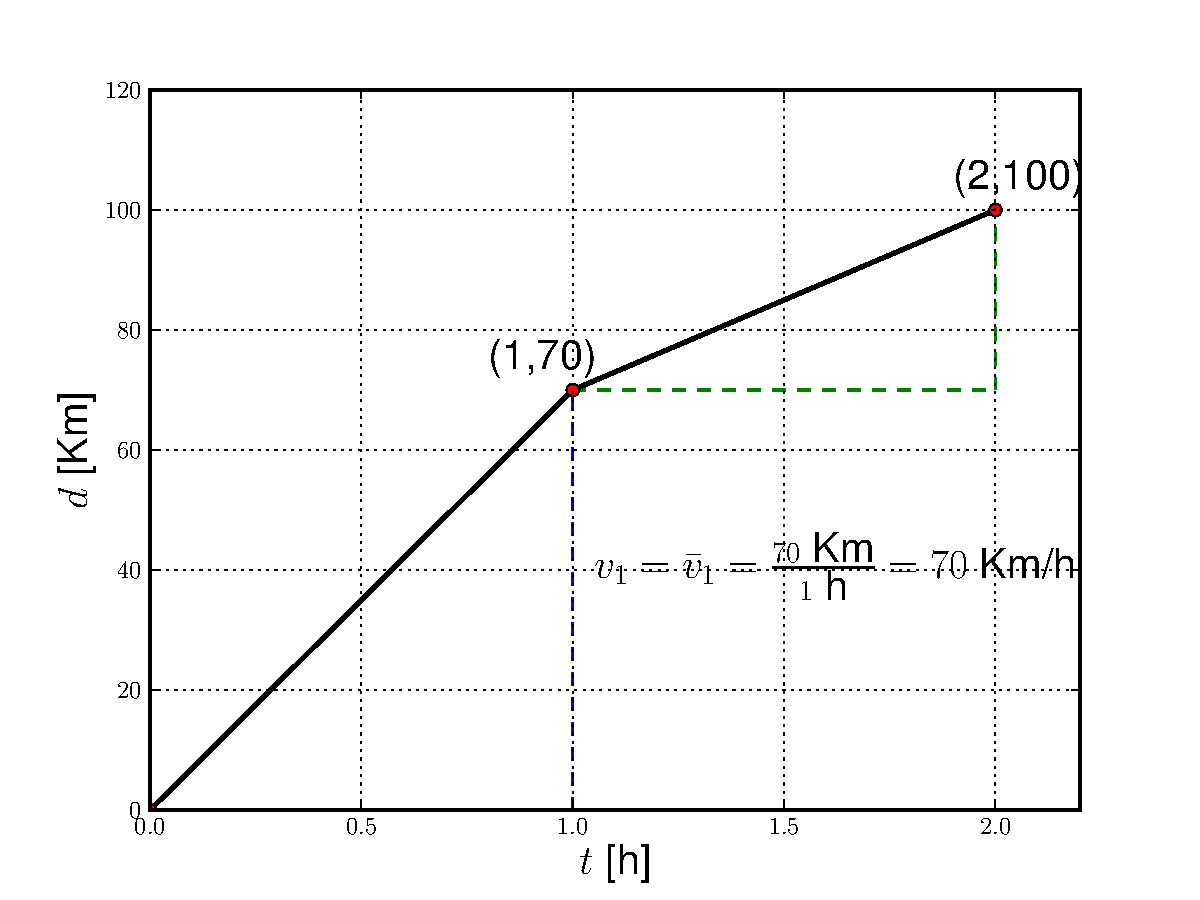
\includegraphics[scale=0.5]{vinstaprom3}
  \caption{Gráfico de distancia versus tiempo}
  \label{fig:vinstaprom3}
\end{figure}
\end{frame}


La rapidez instantánea es la rapidez del carro en un instante particular. Para encontrarla debemos observar una distancia corta en la que el carro se mueva en un intervalo de tiempo muy corto, digamos que una centesima de segundo. Si durante algún momento de la segunda hora el carro se mueve 0.0833 metros en 0.01 segundos, su rapidez instantanea es:
\begin{align}
  v=0.0833/0.01=\SI{8.33}{\meter\per\second} \,,
\end{align}
que en \si{\kilo\meter\per\hour}\ corresponde a
\begin{align}
  v=8.33\ \frac{\cancel{\si{\meter}}}{\cancel{\si{\second}}}\frac{3600\ \cancel{\si{\second}}}{\SI{1}{\hour}}\frac{\SI{1}{\kilo\meter}}{1000\ \cancel{\si{\meter}}}=\SI{30}{\kilo\meter\per\hour}\,.
\end{align}
que corresponde a la pendiente de la línea recta en el segundo
trayecto en la figura~\ref{fig:vinstaprom3}. De hecho, a rapidez
constante, la rapidez promedio coincide con la rapidez instantánea. En
general, para un movimiento en una dimensión, la rapidez instantánea
coincide con la pendiente de la curva en el gráfico distancia con
respecto al tiempo.

\section{Movimiento en varias dimensiones}

\subsection{Vector de Posición}
Nuestra segunda aplicaci\'on de vectores ser\'a la descripci\'on  de la posici\'on y movimiento de un punto en el espacio en tres dimensiones. 

La posici\'on de un punto en el espacio: $(x_1,y_1,z_1)$ no representa un vector. Sin embargo, si movemos el punto a alguna nueva posici\'on, $(x_2,y_2,z_2)$, entonces el desplazamiento define un vector 
\begin{align}
  \Delta \mathbf{r}=\mathbf{r}_2-\mathbf{r}_1
\end{align}
$\Delta\mathbf{r}$ significa ``cambio de $\mathbf{r}$'' o $\mathbf{r}_2-\mathbf{r}_1$ (desplazamiento)

$\Delta t$ significa ``cambio de $t$'' or $t_2-t_1$ (intervalo de tiempo)

El símbolo $\Delta$ (delta) siempre significa ``final menos inicial''

\begin{align}
  \Delta\mathbf{r}=(x_2-x_1,y_2-y_1,z_2-z_1)\,.
\end{align}
$\Delta\mathbf{r}$ es un vector verdadero, aunque los valores de la coordenadas inicial y final dependen del sistema de coordenadas, $\Delta\mathbf{r}$ no depende del sistema de coordenadas. 

$\Delta\mathbf{r}$ tiene las dimensiones f\'\i sicas de longitud. 

%hablar de un ejemplo concreto como el de la abeja de MI Fig. 1.31

El vector de desplazamiento apunta desde la posición inicial hacia la posición final (final menos inicial).

%calcular el desplazamiento númerico de la abeja

Aunque los vectores definen desplazamientos en lugar de posiciones, es posible describir la posici\'on de un punto con respecto al origen de un sistema de coordenadas dado por un vector especial, conocido como el \emph{vector de posici\'on}, que se extiende desde el origen hasta el punto de inter\'es. Usaremos el s\'\i mbolo $\mathbf{r}$ para denotar el vector de posici\'on. La posici\'on de un punto arbitrario $P$ se escribe como
\begin{align}
  \mathbf{r}=(x,y,z)=x\hat{\mathbf{i}}+
  y\hat{\mathbf{j}}+z\hat{\mathbf{k}}\,.
\end{align}

A diferencia de los vectores ordinarios, $\mathbf{r}$ depende del sistema de coordenadas. Si $\mathbf{R}$ es el vector desde el origen de un sistema de coordenadas no primado al origen de un sistema de coordenadas primado, tenemos
\begin{inprogress}
  Escribir los detalles...
\end{inprogress}
\begin{align}
  \mathbf{r}'=\mathbf{r}-\mathbf{R}\,.
\end{align}
\begin{frame}
  Un verdadero  vector es independiente del sistema de coordenadas. Como se muestra en la figura~\ref{fig:vpos},
\begin{align}
  \Delta\mathbf{r}=&\mathbf{r}_2-\mathbf{r}_1\nonumber\\
  =&\mathbf{\mathbf{r}_2'+\mathbf{R}}
-\mathbf{\mathbf{r}_1'+\mathbf{R}}\nonumber\\
=&\mathbf{r}_2'-\mathbf{r}'_1\,.
\end{align}
\end{frame}
\begin{frame}[plain]
  \begin{figure}
  \centering
  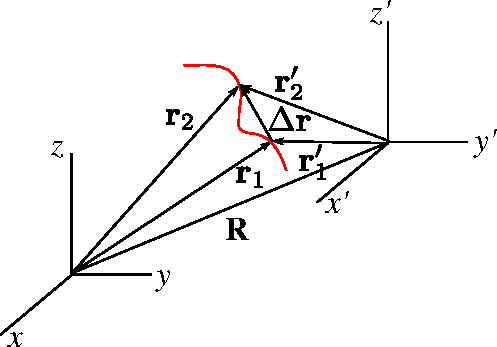
\includegraphics[scale=0.85]{deltar3d}
  \caption{Vector de desplazamiento. (Sec 1.6 \cite{Kleppner})}
  \label{fig:vpos}
\end{figure}
\end{frame}

\subsection{Determinando la velocidad promedio desde un cambio en la posición}
La posici\'on instant\'anea de una part\'\i cula a un tiempo $t_i$ es
\begin{align}
  \mathbf{r}(t_1)=(x(t_1),y(t_1),z(t_1))\qquad \text{\'o}\qquad
  \mathbf{r}_1=(x_1,y_1,z_1)\,,
\end{align}
donde $x_1$ es el valor de $x$ en $t=t_1$, y as\'\i{} sucesivamente. Al tiempo $t_2$ la posici\'on es
\begin{align}
  \mathbf{r}_2=(x_2,y_2,z_2)\,.
\end{align}
El desplazamiento de la part\'\i cula entre los tiempos $t_1$ y $t_2$ es
\begin{align}
  \mathbf{r}_2-\mathbf{r}_1=(x_2-x_1,y_2-y_1,z_2-z_1)\,.
\end{align}



\begin{inprogress}
Pasar las notas del cuaderno de MI aquí.

Escribir los detalles %t_1=t Delta t=t_2-t-> t_2=t+Delta t
\end{inprogress}
El desplazamiento de una part\'\i cula entre los tiempos $t$ y un tiempo posterior $t+\Delta t$ es
\begin{align}
  \Delta\mathbf{r}=\mathbf{r}(t+\Delta t)-\mathbf{r}(t)\,.
\end{align}


\begin{inprogress}
  Fig pag 15 of Kleppner.
\end{inprogress}

\begin{itemize}
\item[Ejemplo]: En dos dimensiones, esta ecuaci\'on es equivalente a
  \begin{align}
    \Delta x=&x(t+\Delta t)-x(t)\nonumber\\
    \Delta y=&y(t+\Delta t)-y(t)\,.
  \end{align}
  como se muestra en la figura~\ref{fig:deltar}
  \begin{figure}
    \centering
    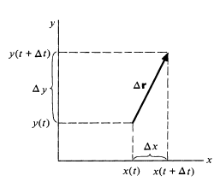
\includegraphics[scale=0.55]{deltar}
    \caption{Desplazamieto entre $t_1$ y $t_2$ (Sec 1.6~\cite{Kleppner})}
    \label{fig:deltar}
  \end{figure}

\end{itemize}


\begin{itemize}
\item[\textbf{Ejemplo:}] Considere una abeja volando. En un tiempo inicial el vector de posición de la abeja es
  \begin{align}
    \mathbf{r}_i=(2,4,0)\si{\meter},\qquad t_i=0\,,
  \end{align}
$\SI{0.1}{\second}$ después, la posición es
\begin{align}
  \mathbf{r}_f=(3,3.5,0)\si{\meter},\qquad t_f=0.1\si{\second}\,.
\end{align}
Realice un diagrama de la situación y encuentre
\begin{enumerate}
\item la velocidad promedio
  \label{item:abejaa}
\item La rapidez promedio
  \label{item:abejab}
\item La dirección de la velocidad promedio
  \label{item:abejac}
\end{enumerate}
\begin{itemize}
\item[\ref{item:abejaa}.] 

\begin{align*}
  \mathbf{v}_{\text{prom}}=(10,-5,0)\si{\meter\per\second}\,.
\end{align*}

\item[\ref{item:abejab}.]
\begin{align*}
  v_{\text{prom}}=\SI{11.18}{\meter\per\second}\,.
\end{align*}
\item[\ref{item:abejac}.]
  \begin{align*}
    \hat{\mathbf{v}}_{\text{prom}}=\frac{\mathbf{v}_{\text{prom}}}{v_{\text{prom}}}=(0.804,-0.447,0)
  \end{align*}

\end{itemize}
\end{itemize}

\subsection{Velocidad instantánea}

Considere la curva en la figura \ref{fig:flyingball1a}. Los puntos de color rojo marcan la posición de una bola a intervalos de tiempo de un segundo. Mientras que la bola está en el aire, su velocidad está constantemente cambiando, debido a las interacciones con la tierra (gravedad) y con el aire (resistencia del aire). 
\begin{figure}
  \centering
  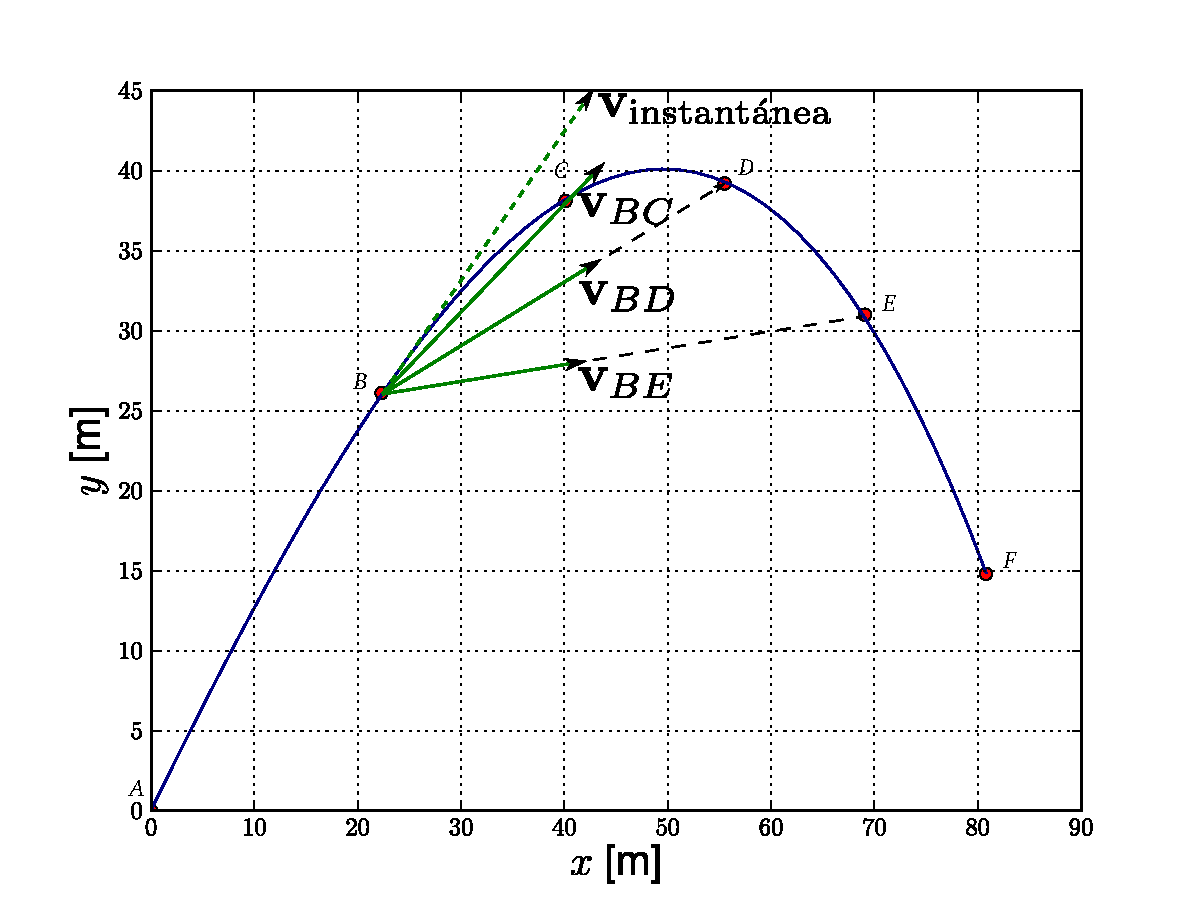
\includegraphics[scale=0.4]{flyingball1a}
  \caption{Movimiento de una bola}
  \label{fig:flyingball1a}
\end{figure}

Suponga que hacemos la pregunta: ¿cual es el valor de la velocidad en el instante preciso que alcanza el punto $B$?. Está cantidad debería llamarse la velocidad instantánea. Podemos aproximar la velocidad instantánea de la bola, encontrando su velocidad promedio sobre un intervalo de tiempo más grande. 

La Tabla muestra el vector de posición de la bola a diferentes tiempos en los puntos ilustrados en la figura~\ref{fig:flyingball1a}.

\begin{table}
  \centering
  \begin{tabular}{lll}
    loc. & $t\ (\text{s})$ & Posición (m)\\\hline
    $A$ & $0.0$ &$0,0,0$ \\
    $B$ & $1.0$ &$(22.3,26,1,0)$ \\
    $C$ & $2.0$ &$(40.1,38.1,0)$ \\
    $D$ & $3.0$ &$(55.5,39.2,0)$ \\
    $E$ & $4.0$ &$(69.1,31.0,0)$ \\
    $F$ & $5.0$ &$(80.8,14.8,0)$ \\\hline
  \end{tabular}
  \caption{Tabla mostrando el tiempo transcurrido y la posición de la bola en cada posición de la figura~\ref{fig:flyingball1a}}
  \label{tab:flyingball1a}
\end{table}

\begin{align}
  \mathbf{v}_{EB}=&\frac{\Delta \mathbf{r}_{EB}}{\Delta t}
=\frac{\mathbf{\mathbf{r}_E-\mathbf{r}_B}}{t_E-t_B}=
\frac{[(69.1,31.0,0)-(22.3,26,1,0)]\ \text{m}}{(4.0-1.0)\ \text{s}}\nonumber\\
=&(15.6,1.6,0)\ \frac{\text{m}}{\text{s}}\nonumber\\
  \mathbf{v}_{DB}=&\frac{\Delta \mathbf{r}_{DB}}{\Delta t}
=\frac{\mathbf{\mathbf{r}_D-\mathbf{r}_B}}{t_D-t_B}=
\frac{[(55.5,39.2,0)-(22.3,26,1,0)]\ \text{m}}{(3.0-1.0)\ \text{s}}\nonumber\\
=&(16.6,6.55,0)\ \frac{\text{m}}{\text{s}}\nonumber\\
  \mathbf{v}_{CB}=&\frac{\Delta \mathbf{r}_{CB}}{\Delta t}
=\frac{\mathbf{\mathbf{r}_C-\mathbf{r}_B}}{t_C-t_B}=
\frac{[(40.1,38.1,0)-(22.3,26,1,0)]\ \text{m}}{(2.0-1.0)\ \text{s}}\nonumber\\
=&(17.8,12.0,0)\ \frac{\text{m}}{\text{s}}\,,
\end{align}

\begin{align}
  v_{EB}=&15.7\ \frac{\text{m}}{\text{s}}\nonumber\\
  v_{DB}=&17.8\ \frac{\text{m}}{\text{s}}\nonumber\\
  v_{CB}=&21.5\ \frac{\text{m}}{\text{s}}\,,
\end{align}
%mejorar redacción
¿cual aproxima mejor la velocidad instantánea (figura~\ref{fig:flyingball8})?

\begin{figure}
  \centering
  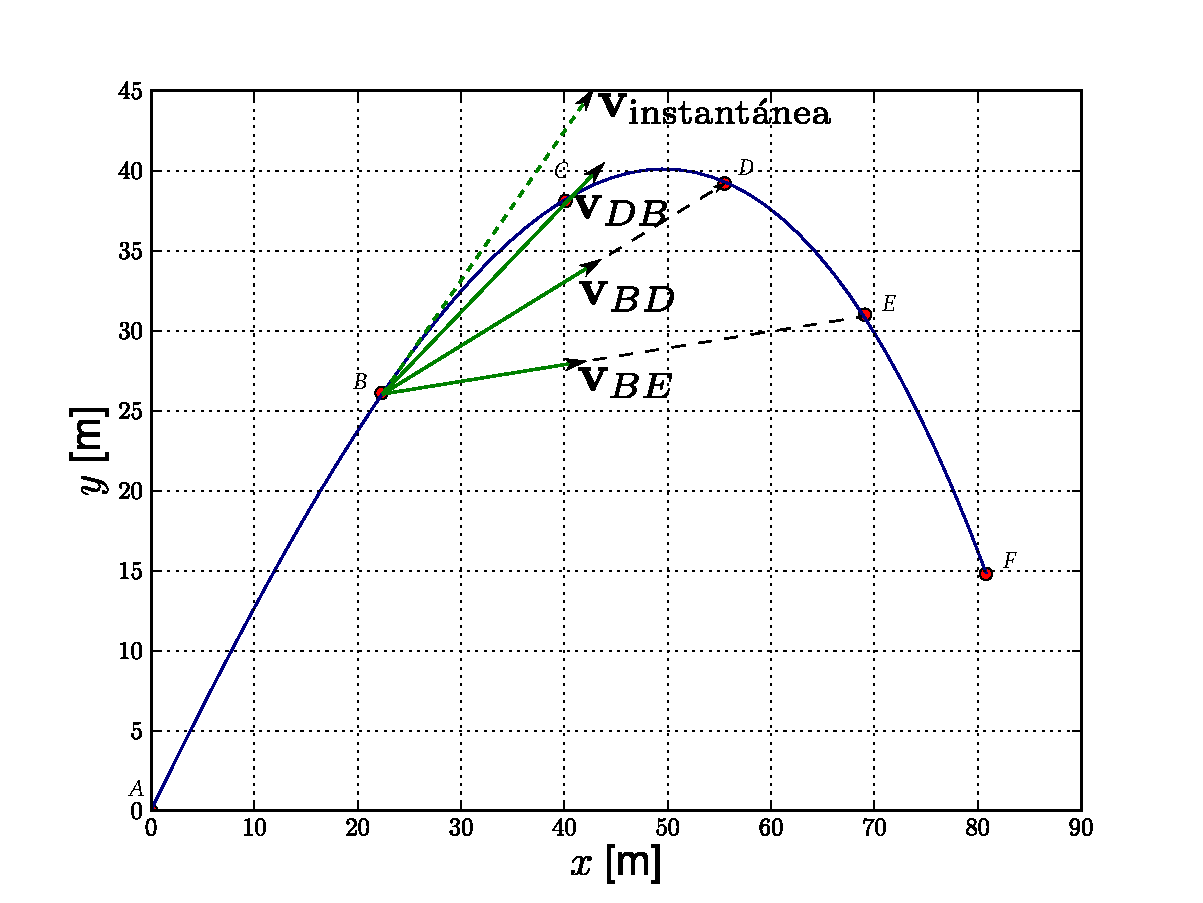
\includegraphics[scale=0.4]{flyingball8}
  \caption{Moviemto de una bola}
  \label{fig:flyingball8}
\end{figure}


La velocidad $\mathbf{v}$ de la partícula a medida que ésta se mueve a lo largo de una trayectoria se define como
\begin{align}
  \mathbf{v}=&\lim_{\Delta t\to0}\frac{\Delta\mathbf{r}}{\Delta t}\nonumber\\
  &=\frac{d\mathbf{r}}{dt}\,,
\end{align}
que es equivalente a las ecuaciones escalares
\begin{align}
  v_x=&\lim_{\Delta t\to0}\frac{\Delta x}{\Delta t}=\frac{dx}{dt}\nonumber\\
  v_y=&\lim_{\Delta t\to0}\frac{\Delta y}{\Delta t}=\frac{dy}{dt}\nonumber\\
  v_z=&\lim_{\Delta t\to0}\frac{\Delta z}{\Delta t}=\frac{dz}{dt}\,.
\end{align}

La notaci\'on vectorial permite describir el movimiento en tres dimensiones con una sola ecuaci\'on, una econom\'\i a muy grande comparada con las tres ecuaciones que tocar\'\i a escribir si se tuviese que hacer de otro modo. 

Alternativamente, ya que $\mathbf{r}=x\hat{\mathbf{i}}+
y\hat{\mathbf{j}}+z\hat{\mathbf{k}}$, obtenemos por simple
diferenciaci\'on que (los vectores unitarios pueden cambiar bajo
diferenciaci\'on en otros sistemas de coordenadas diferentes al
cartesiano)
\begin{align}
 \frac{d\mathbf{r}}{dt}=&\frac{dx}{dt}\hat{\mathbf{i}}   
+\frac{dy}{dt}\hat{\mathbf{j}}   +\frac{dz}{dt}\hat{\mathbf{k}}\nonumber\\
=&
\left(
\frac{dx}{dt},\frac{dy}{dt},\frac{dz}{dt}
\right)\nonumber\\
=&(v_x,v_y,v_z)
\end{align}
%como antes.




En el l\'\i mite $\Delta t\to0$, $\Delta\mathbf{r}$ se convierte en la tangente a la trayectoria, como se \'\i ndica en la figura~\ref{fig:flyingball8}. Sin embargo, la relaci\'on
\begin{align}
  \label{eq:Drvt}
  \Delta\mathbf{r}\approx&\frac{d\mathbf{r}}{dt}\Delta t\nonumber\\
  \Delta\mathbf{r}=&\mathbf{v}\Delta t,
\end{align}
que llega a ser exacta en el l\'\i mite $\Delta t\to 0$, muestra que $\mathbf{v}$ es paralelo a $\Delta\mathbf{r}$; la velocidad instant\'anea $\mathbf{v}$ de una part\'\i cula es en todas partes tangente a la trayectoria. 

%sigue en el cuaderno

La ec.~\eqref{eq:Drvt} puede reescribirse en la forma
\begin{align*}
  \mathbf{r}_2-\mathbf{r}_1=\mathbf{v}_{\text{prom}}(t_2-t_1)\,,
\end{align*}
de modo que el vector de desplazamiento es el promedio del vector de velocidad en el intervalo de tiempo.

Si conocemos la velocidad, tenemos una relación para actualizar la posición a partir de una posición inicial $\mathbf{r}_1$
\begin{align*}
  \mathbf{r}_2=&\mathbf{r}_1+\mathbf{v}_{\text{prom}}(t_2-t_1)\nonumber\\
=&\mathbf{r}_1+\mathbf{v}_{\text{prom}}\Delta t\,.
\end{align*}
Si se conoce la posición inicial, la velocidad promedio y el intervalo temporal, entonces podemos predecir la siguiente posición del movimiento.

Esta aproximación puede llegar a funcionar muy bien para intervalos de
tiempo pequeños pues en tal caso la velocidad promedio es muy similar
a la velocidad instantánea. De este forma, para simular el movimiento
de un cuerpo por complicado que sea, es suficiente ir actualizando su
posición a través de la velocidad promedio, si podemos garantizar que
el intervalo de tiempo es suficientemente pequeño.

\ejemplo{}
\begin{frame}[plain]
A un tiempo $t_1=\SI{12.18}{\second}$ después de la 1:30~PM el vector de posición de una bola es $\mathbf{r}_1=(20,8,-12)\si{\meter}$ y su velocidad es $\mathbf{v}_{\text{prom}}=(9,-4,6)\si{\meter\per\second}$. A un tiempo $t_2=12.21\si{\second}$ después de la 1:30~PM: ¿donde está la bola?, asumiendo que la velocidad no cambie en el corto intervalo de tiempo.

  
  \begin{align*}
  \mathbf{r}_2=&\mathbf{r}_1+\mathbf{v}_{\text{prom}}(t_2-t_1)\nonumber\\
  =&(20,8,-12)\si{\meter} +  \left[(9,-4,6)\si{\meter\per\second}\right](12.21-12-18)\si{\second}\nonumber\\
  =&(20,8,-12)\si{\meter}+(0.27,-0.12,0.18)\si{\meter}\nonumber\\
=&(20.27,7.88,-11.82)\si{\meter}\,.
  \end{align*}
\end{frame}
\finejemplo


\ejemplo{}
\textbf{Encontrando $\mathbf{v}$ a partir de $\mathbf{r}$}\\
La posici\'on de una part\'\i cula est\'a dada por
\begin{align}
  \mathbf{r}=A(e^{\alpha t}\hat{\mathbf{i}}+e^{-\alpha t}\hat{\mathbf{j}})\,,
\end{align}
donde $\alpha$ es constante. Encuentre la velocidad y bosqueje la trayectoria.
\begin{align}
    \mathbf{v}=&\frac{d\mathbf{r}}{dt}\nonumber\\
    =&A(\alpha e^{\alpha t}\hat{\mathbf{i}}-\alpha e^{-\alpha t}\hat{\mathbf{j}})\,,
\end{align}
o
\begin{align}
  v_x=&A\alpha e^{\alpha t}\nonumber\\
  v_y=&-A\alpha e^{-\alpha t}\,.
\end{align}
La magnitud de $\mathbf{v}$ es
\begin{align}
  v=&\sqrt{v_x^2+v_y^2}\nonumber\\
  =&A\alpha\sqrt{e^{2\alpha t}+e^{-2\alpha t}}\,.
\end{align}

\begin{inprogress}
  Pasar los ejemplo de MI desarrollados en el cuaderno
\end{inprogress}
%Al describir el movimiento de un punto, es usualmente útil considerar los casos l\'\i mite:
\finejemplo

\subsection{Aceleración}

Aceleración promedio:
\begin{align}
  \mathbf{a}_{\text{prom}}=&\frac{\Delta \mathbf{v}}{\Delta t}
\end{align}

Aceleración instantánea
\begin{align}
  \mathbf{a}=&\lim_{\Delta t\to 0}\frac{\Delta \mathbf{v}}{\Delta t}=\frac{d\mathbf{v}}{dt}
\end{align}
%continua en las notas del cuaderno

\subsection{Moméntum}

La primera Ley de Newton no permite hacer predicciones cuantitativas. Para hacer estas predicciones se requiere una medida que cuantifique los efectos de la interacciones. Surge entonces la pregunta: ¿qué factores hacen difícil o fácil cambiar la velocidad de un objeto?

Probablemente habrá notado que si dos objetos tienen la misma velocidad pero uno es más liviano que el otro, es más difícil cambiar la velocidad del objeto más masivo. 

\begin{frame}[plain]
  \begin{quote}
  Es más fácil detener una bola de beisbol viajando a $\SI{100}{\kilo\meter\per\hour}$, que un camión viajando a $\SI{100}{\kilo\meter\per\hour}$

Es más fácil cambiar la dirección de una canoa que la dirección del Titanic.
\end{quote}
\end{frame}

Una cantidad que se puede entonces asociar con el cambio de movimiento de un cupero es el \emph{moméntum} o \emph{cantidad de movimiento} instantáneo de una partícula de masa $m$ moviendo con velocidad instantánea $\mathbf{v}$
\begin{align}
  \mathbf{p}=&\gamma m \mathbf{v}\,, &\text{donde: } \gamma=&\frac{1}{\sqrt{1-{|\mathbf{v}|^2}/{c^2}}}\,,
\end{align}
y $c\approx 3\times 10^8\ $m/s es la velocidad de la luz.

Si $\gamma\approx1$, o equivalentemente, si $|\mathbf{v}|\ll c$:
\begin{align}
  \mathbf{p}\approx &m \mathbf{v}
\end{align}


\begin{extrapage}
  \newpage
  
  \qquad
  \newpage
\end{extrapage}

%%% Local Variables: 
%%% mode: latex
%%% TeX-master: "mecanica"
%%% End: 

